 \chapter{Literature review}

\section{USAR Robots}

\begin{wrapfigure}{r}{0.35\textwidth} %this figure will be at the right
	\centering
	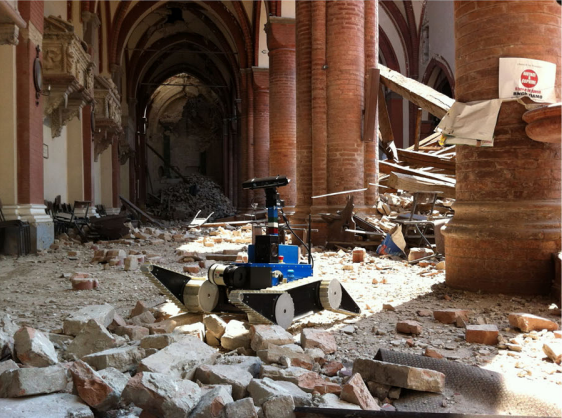
\includegraphics[width=0.35\textwidth]{stateof-tracked}
	\caption{A tracked USAR robot, with paddles for obstacle climbing \citep{stateof}}
	\label{stateof tracked}
\end{wrapfigure}

In both natural and man-made disasters, USAR operations are critical for reducing casualties. Robots can be deployed in USAR operations to complement human and canine rescuers. Robots have the advantage of being able to be deployed in scenarios too small or too dangerous for humans, and aerial robots such as quadcopters are extremely effective at quickly mapping terrain and providing situational awareness to teams. Other emerging applications of USAR robotics are remote fire fighting, victim interaction and extraction \citep{stateof}.\\

\begin{wrapfigure}{l}{0.35\textwidth} %this figure will be at the left
	\centering
	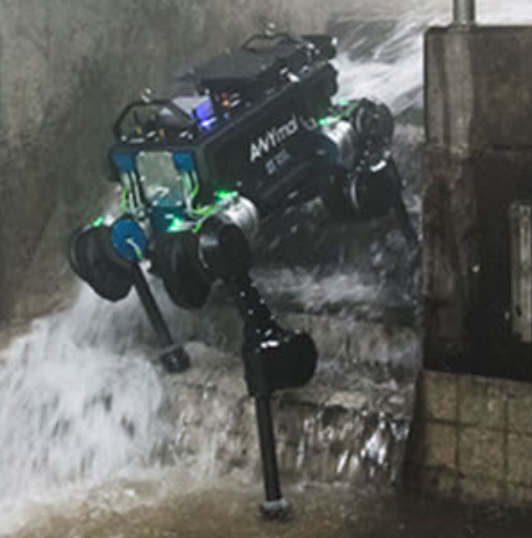
\includegraphics[width=0.35\textwidth]{stateof-wheelleg}
	\caption{ANYmal, a legged USAR robot \citep{stateof}}
	\label{stateof wheelleg}
\end{wrapfigure}

In order to perform USAR operations, robots need some form of locomotion. For ground robots, this typically involves either tracks, wheels, or legs. \citep{stateof}. Tracked robots with actuated paddles for obstacle climbing, such as the one shown in Figure \ref{stateof tracked}, have been found to perform extremely well. This is evident by their representation in the winners of the Robocup Rescue Robot League (RRL), an event in which teams compete to produce robots for versatile USAR operations \citep{Sheh-2016}. Wheeled robots are generally the simplest and easiest to repair, but can get stuck more easily in uneven terrain. Legged robots provide the advantage of not needing a continuous path, and rapid developments in optical sensors and control systems are enabling them to be even more viable, one of these robots is shown in Figure. Wheel-leg hybrid systems will use legged motion for navigating difficult terrain, and wheels when on smooth ground \citep{stateof}. 

\section{Load-Intuitive Modules} %~~~~~~~~~~~~~~~~~~~~~~~~~~~~~~~~~~~~~~~~~~~~~~~~~~~~~~~~~~~~~~

\begin{wrapfigure}{r}{0.35\textwidth} %this figure will be at the right
	\centering
	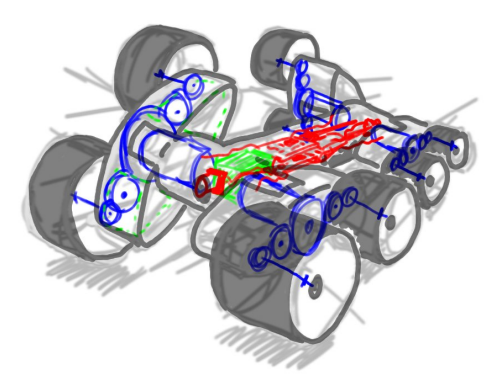
\includegraphics[width=0.35\textwidth]{Wilson-sketch}
	\caption{Systems layout of Wilson's LIM device \citep{Wilson-2013}}
	\label{Wilson sketch-lit}
\end{wrapfigure}

A Load-Intuitive Module (LIM) refers to a wheel system proposed by Matthew Wilson, shown in Figure \ref{Wilson sketch-lit} \citep{Wilson-2013}. The LIM system uses a two outer "minor wheels" placed on a central hub that can be rotated as a "major wheel". The minor wheels are geared to the central hub such that they drive the vehicle, however if they experience high resistance, for example from hitting an obstacle, the torque will cause the major wheel to rotate instead, flipping one of the minor wheels over the obstacle to automatically climb it. The system is referred to as "Load-Intuitive" because it will intuitively climb over obstacles in response to increased load on the wheels. LIMs are designed to be used in low cost USAR robots, allowing them to climb over objects without the need for many actuators.\\

One advantage LIMs provide over existing locomotion methods is that they can climb obstacles higher than their profile, meaning they can enter low voids while rolling, and climb relatively tall obstacles by flipping over them. Another advantage is that LIMS require minimal actuation, one motor can be used to drive both the rolling and flipping motion, which will reduce costs when compared with other designs.\\

\noindent "LIMed" robot platforms (platforms using LIMs for locomotion) were built individually by four final year students at UCT \citep{Wilson-2013}, \citep{Haskel-2017}, \citep{Buchanan-2018}, and \citep{Powrie-2019}. These platforms show some success in climbing a single step, albeit inconsistently.

\subsection{Wilson's LIM robot} %~~~~~~~~~~~~~~~~~~~~~~~~~~~~~~~~~~~~~~~~~~~~~~~~~~~~~~~~~~~~~~~~~~~~~~~~~~~~~~~~

\begin{wrapfigure}{r}{0.35\textwidth}
	\centering
	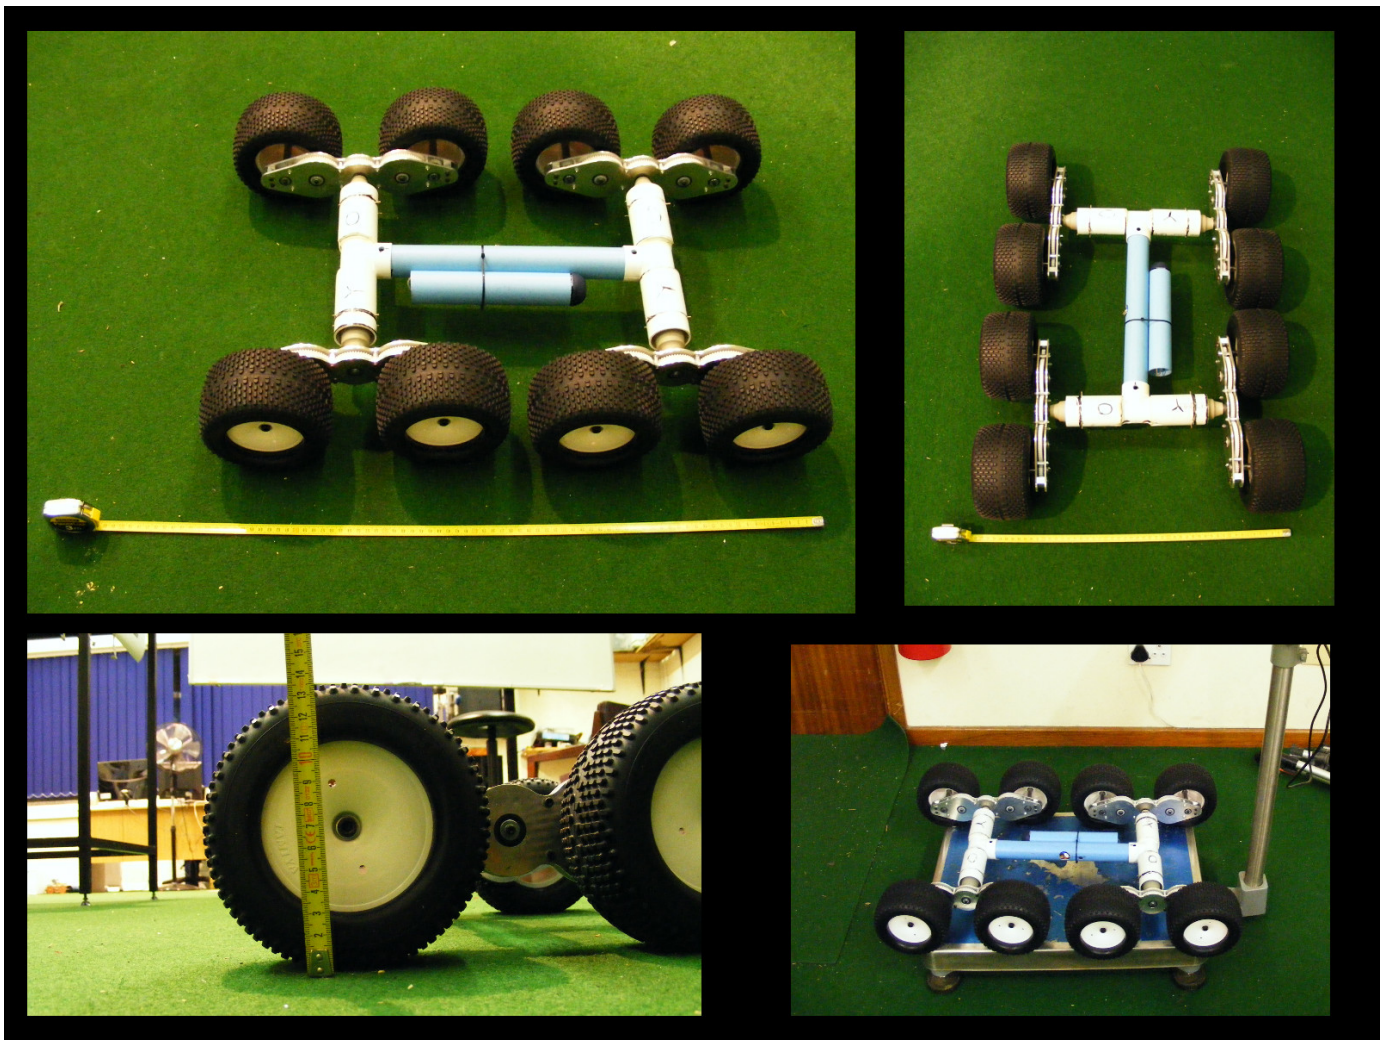
\includegraphics[width=0.35\textwidth]{Wilson-robot}
	\caption{Wilson's Robot \citep{Wilson-2013}}
	\label{Wilson robot}
\end{wrapfigure}

Wilson designed and built the first LIM robot in 2013, shown in Figure \ref{Wilson robot}. This robot was designed as a prototype for a low cost USAR stair-climbing robot. At first Wilson considered only using LIMs for the front set of wheels, with the rear set using regular wheels. However, after performing a 2D simulation in Algodoo, he concluded that using LIMs for the rear wheels was necessary as regular wheels provided little to no support to the climbing motion after the first step, presumably because the rear wheel would stop making contact with the stairs. Using LIMs for the rear wheels means they will be able to climb as well, and can always apply a forward force on the body.



\begin{wrapfigure}{l}{0.35\textwidth}
	\centering
	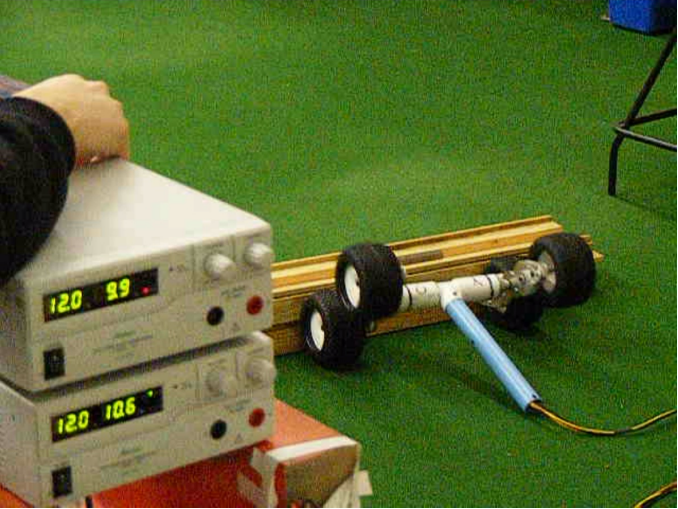
\includegraphics[width=0.35\textwidth]{Wilson-climbing}
	\caption{Wilson's half assembly climbing a stair \citep{Wilson-2013}}
	\label{Wilson climbing}
\end{wrapfigure}

Wilson's robot had some limitations that prevented him from performing extensive tests. Chiefly, it was unable to climb stairs as the motors would stall upon encountering an obstacle. To validate the LIM concept in spite of this issue, Wilson split the robot in half and tested stair climbing using only the front LIMs and the chassis dragging behind as a tail. This "tail-dragging half assembly" was able to climb a single step as shown in Figure \ref{Wilson climbing}. Wilson's project ran out of time before he was able to solve the climbing motion of the complete robot, however he was able to confirm that the LIM system can climb at least a single stair in the half assembly configuration \citep{Wilson-2013}.

\subsection{Haskel's Theseus} %~~~~~~~~~~~~~~~~~~~~~~~~~~~~~~~~~~~~~~~~~~~~~~~~~~~~~~~~~~~~~~~~~

\begin{wrapfigure}{r}{0.35\textwidth}
	\centering
	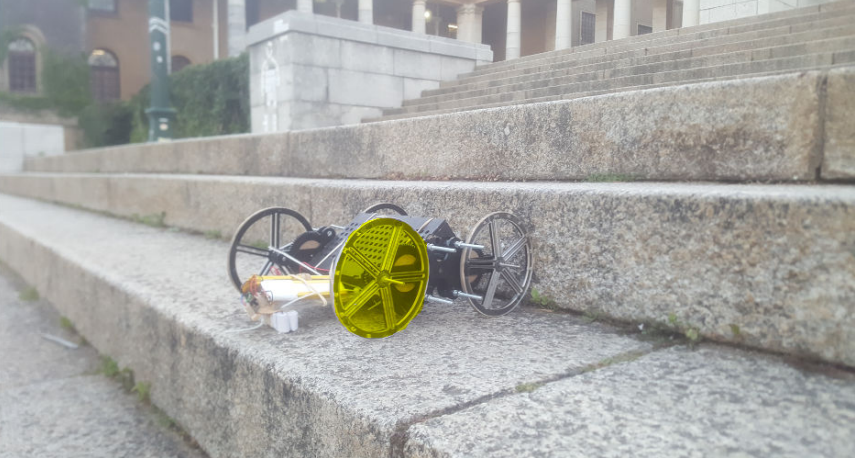
\includegraphics[width=0.35\textwidth]{Haskel-robot}
	\caption{Haskel's Theseus \citep{Haskel-2017}}
	\label{Haskel robot}
\end{wrapfigure}
Haskel designed and built a LIMed robot to further test the concept, which he named "Theseus", shown in Figure \ref{Haskel robot}. Unlike Wilson, Haskel assumes that using LIMs for rear wheels is not necessary for the stair climbing motion, and instead chooses to use a dragging tail to provide counter torque, similar to the tail-dragging half assembly used by Wilson. Theseus is much smaller and lighter than Wilson's robot.\\

Haskel tested different concepts for the tire tread, dragging tail, and gear ratios. However, none of his configurations could consistently climb a step. In the majority of step-climbing attempts, Theseus' LIMs would flip over to mount the step, but it would not be able to pull itself up. This can be attributed to a lack of grip or a lack of torque. Haskel intended to do further work on the project, however he ran out of time due to component shortages and protests at UCT \citep{Haskel-2017}.
\newpage
\subsection{Buchanan's Ascender} %~~~~~~~~~~~~~~~~~~~~~~~~~~~~~~~~~~~~~~~~~~~~~~~~~~~~~~~~~~~~~~~~~

\begin{wrapfigure}{r}{0.35\textwidth}
	\centering
	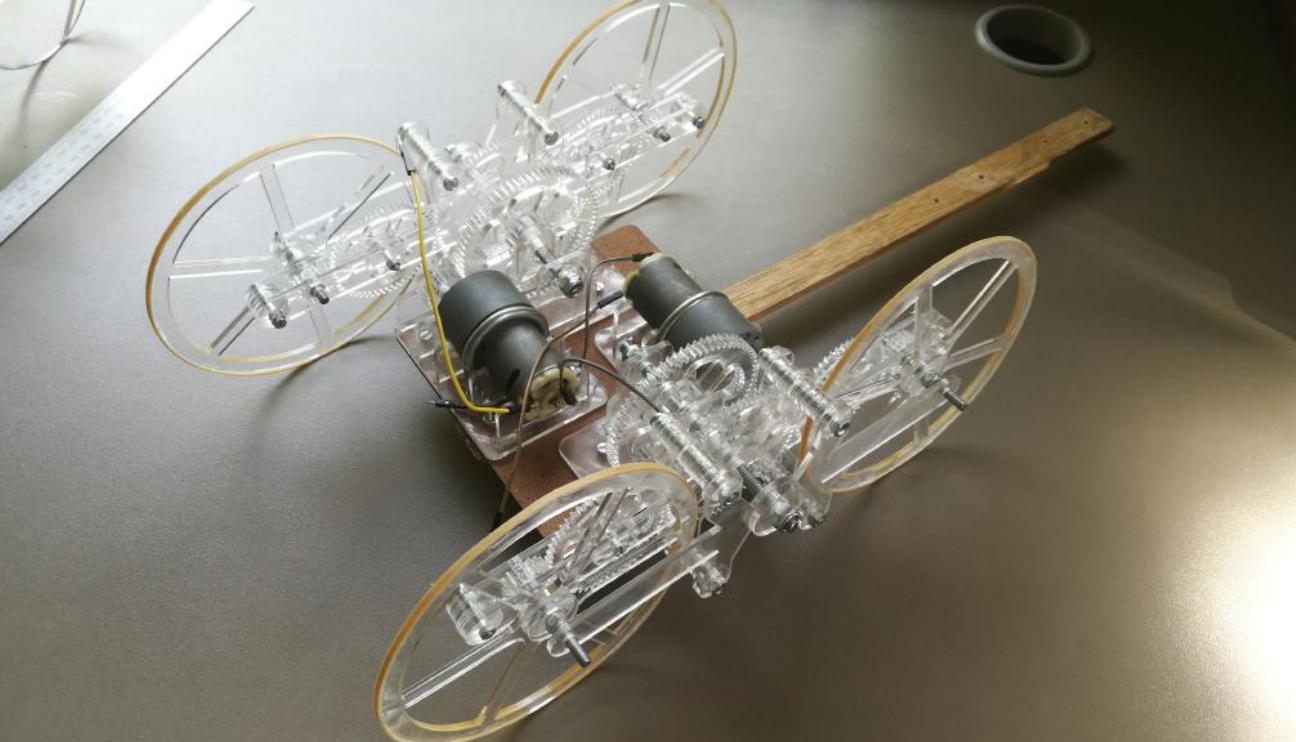
\includegraphics[width=0.35\textwidth]{Buch-robot}
	\caption{Buchanan's Ascender \citep{Buchanan-2018}}
	\label{Buch robot}
\end{wrapfigure}
Buchanan designed and built "Ascender", a robot platform using LIMs for locomotion, shown in Figure \ref{Buch robot}. Buchanan iterated on the design several times in order to reduce mass and increase torque. The intention was to build a drivetrain that could be combined with the electronics of Haskel's Theseus to produce a successful stair climbing robot. As such, the Ascender does not include any electronic control systems, and is instead controlled externally by power supplies connected to the motors.

Buchanan's testing showed that the Ascender was able to climb a single step of 120 mm in 6 out of 10 attempts, and a step of 140mm in 2 out of 10 attempts. Buchanan noted a flaw in the design; after the LIMs flip over as part of the climbing motion, the body of the robot would lodge itself onto the the edge of the step and the wheels would spin freely, a phenomenon referred to as beaching. The LIMs would then spin until the top wheel makes contact with the top of the step, from there it would either grip and pull the robot up the step as intended, or it would dislodge the body and the robot would fall off the step. Buchanan also reported that the Ascender was fragile to the point that it broke during the testing. Buchanan did not test the Ascender's ability to climb a staircase, but he concluded that it would be able to as a staircase is simply repeated single steps. \citep{Buchanan-2018}

\subsection{Powrie's Di-Wheel robot}

\begin{wrapfigure}{r}{0.35\textwidth}
	\centering
	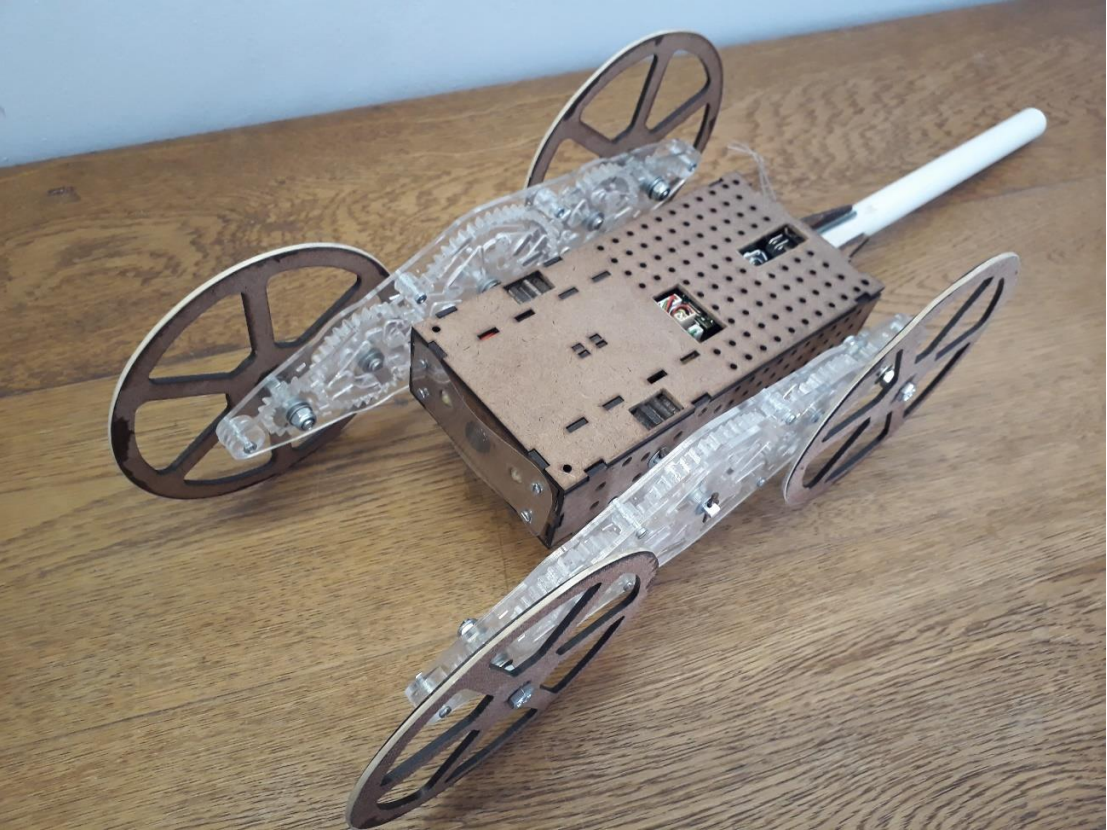
\includegraphics[width=0.35\textwidth]{Powrie-device}
	\caption{Powrie's Di-Wheel Robot \citep{Powrie-2019}}
	\label{fig:Powrie robot}
\end{wrapfigure}
Powrie developed a robot using LIMs, however in his report he referred to LIMs as Di-Wheels. His reason for renaming them is that the behaviour of the LIMs does not only respond to external loads on the wheels, it also depends on the torque applied by the motors. He chose the name "Di-Wheel" in reference to a similar design by the name of "Tri-Wheel", which used three minor wheels instead of two, developed by \cite{Smith-2015}. Powrie's Di-Wheel robot is larger and more robust than Buchanan's Ascender, while being lighter than Wilson's LIMed robot. It is shown in Figure \ref{fig:Powrie robot}.\\


The Di-Wheel robot was successful in climbing a single step of 220 mm. Further testing was not performed as noise from the robot's motors would interfere with the control system, preventing untethered driving. Powrie ran out of time before he was able to solve this issue. Powrie also found that when both motors are powered on, one of the LIMs would flip first, putting all the weight on the other LIM so preventing it from flipping. The result is that the robot would fall on its side, as seen in Figure \ref{Powrie falling} \citep{Powrie-2019}.\\
\begin{figure}[ht]
	\centering
	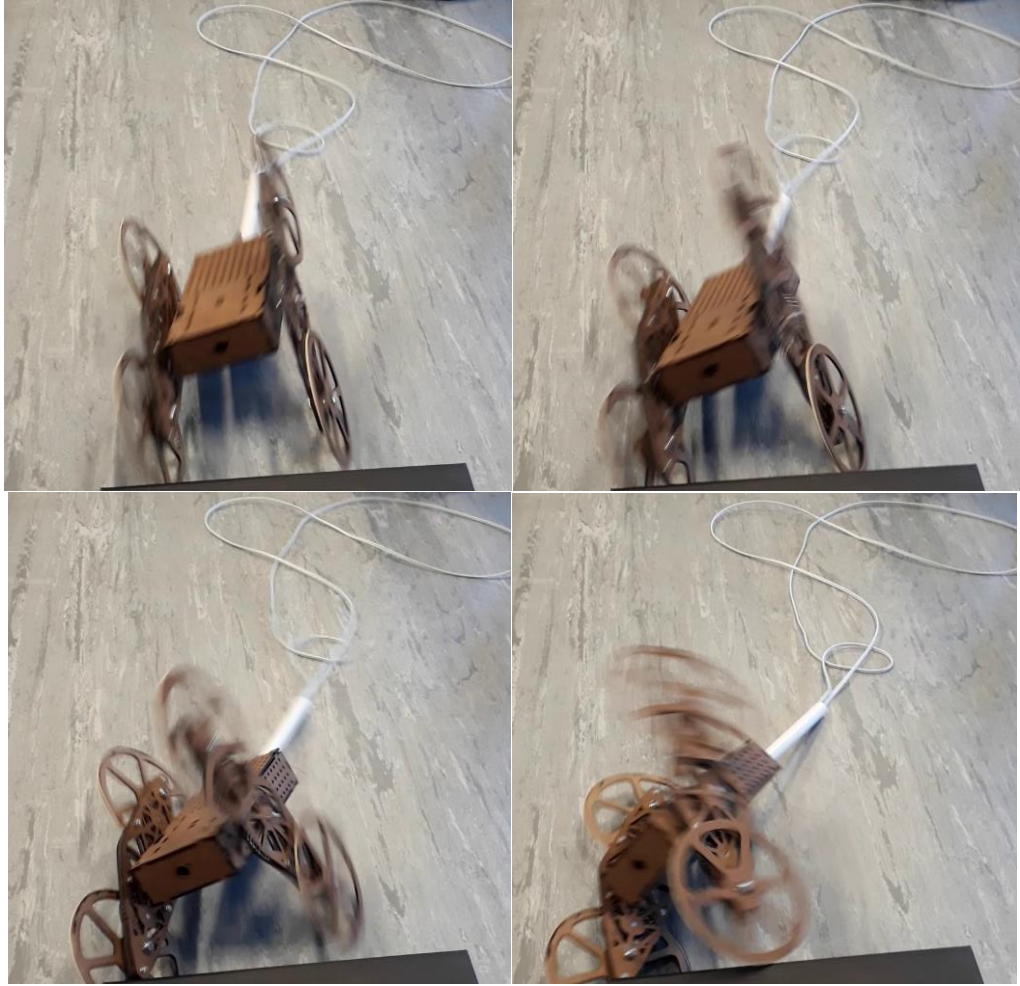
\includegraphics[width=0.35\textwidth]{Powrie-falling}
	\caption{The Di-Wheel robot falling due to unsynchronised LIMs \citep{Powrie-2019}}
	\label{Powrie falling}
\end{figure}


\subsection{Gearing} %~~~~~~~~~~~~~~~~~~~~~~~~~~~~~~~~~~~~~~~~~~~~~~~~~~~~~~~~~~~~~~~~~
%Add drawing!!
The gear ratios of the LIMs will affect its motion significantly. The rotational speed of the central gear will be translated into both the speed of the LIM frame and the speed of the wheels:
\begin{align*}
	\dot{\theta}_{\mathrm{Sun}} &= \dot{\theta}_{\mathrm{Frame}} + \frac{N_\mathrm{Planet}}{N_\mathrm{Sun}}\dot{\theta}_{\mathrm{Planet}} \tag{1}\\
\end{align*}
where $\dot{\theta}_{\mathrm{Sun}}$ is the angular speed of the central gear, $\dot{\theta}_{\mathrm{Frame}}$ is the angular speed of the LIM frame, $\dot{\theta}_{\mathrm{Planet}}$ is the angular speed of the outer gears and wheels relative to the frame, $N_{\mathrm{Planet}}$ is the number of teeth on the outer gears, and $N_\mathrm{Sun}$ is the number of teeth on the central gear.\\

When both the wheels and the LIM frame aren't constrained, the system is under-actuated and its motion is non-trivial. In the case that the LIM frame isn't flipping (i.e. normal driving on a flat plane), $\dot{\theta}_{\mathrm{Frame}} = 0$, therefore:\\
 \begin{align*}
 	\dot{\theta}_{\mathrm{Planet}} &= \frac{N_\mathrm{Sun}}{N_\mathrm{Planet}}\dot{\theta}_{\mathrm{Sun}} \tag{2}\\
 \end{align*}
When the wheels have encountered an obstacle, such as a step, friction will prevent them from turning, $\dot{\theta}_{\mathrm{Planet}} + \dot{\theta}_{\mathrm{Frame}} = 0$. In this case:
\begin{align*}
	\dot{\theta}_{\mathrm{Frame}} &= \frac{\dot{\theta}_{\mathrm{Sun}}}{(1-\frac{N_\mathrm{Planet}}{N_\mathrm{Sun}})} \tag{3}\\
\end{align*}

This means that during flipping motion, if $\frac{N_\mathrm{Planet}}{N_\mathrm{Sun}} > 1$, then the LIM frame will flip in the opposite direction to the rotation of the central gear, so the front wheel will roll up the side of the obstacle \citep{Wilson-2013}. This is ineffective for climbing steps as the LIM will never mount the step, but rather continue rotating backwards until it returns to the starting position \citep{Haskel-2017}.\\

\begin{figure}[h]
	\centering
	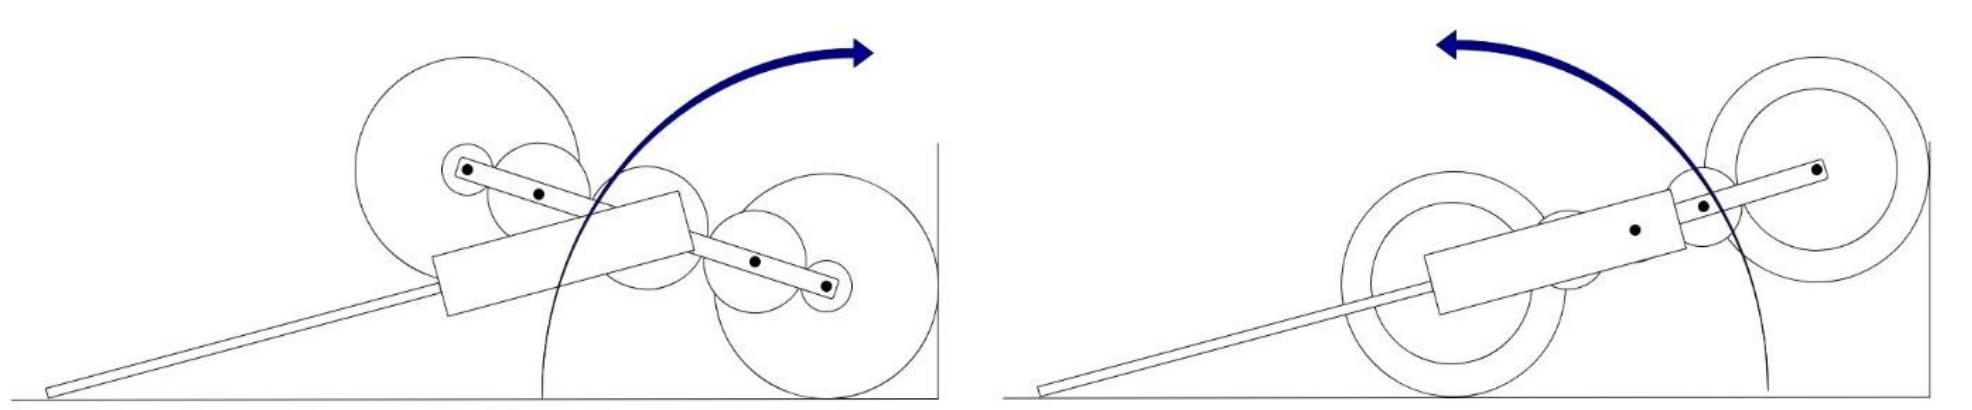
\includegraphics[width=0.9\textwidth]{Powrie-gear-differences}
	\caption{Two different climbing motions using different gear ratios \citep{Powrie-2019}}
	\label{Powrie gears}
\end{figure}

If $\frac{N_\mathrm{Planet}}{N_\mathrm{Sun}} < 1$, then the LIM frame will rotate forward, the rear wheel will flip over and mount the obstacle. This allows the LIM to climb stairs as intended.\\
The two cases are shown in Figure \ref{Powrie gears}, with the left showing the case when $\frac{N_\mathrm{Planet}}{N_\mathrm{Sun}} < 1$, and the right showing the case when $\frac{N_\mathrm{Planet}}{N_\mathrm{Sun}} > 1$.



\subsection{Control requirements} %~~~~~~~~~~~~~~~~~~~~~~~~~~~~~~~~~~~~~~~~~~~~~~~~~~~~~~~~~~~~~~~~~

LIMs are considered "Load intuitive" because of their ability to adapt to terrain mechanically. Open-loop control is ideal in this case, as an operator need only turn the motor on and the LIM will drive forward if it can, or attempt to climb an obstacle if it is obstructed \citep{Wilson-2013}. However, Powrie found that his robot was not suited to open loop control. When full voltage is provided to the motor, the LIMS would flip even if when is on a flat plane. Powrie's calculations suggest that whether the LIM flips or not is largely dependent on the torque applied to it. A low torque results rolling, and a high torque results in flipping. His report suggests that LIMs only responds to terrain intuitively for a "medium torque" \citep{Powrie-2019}. In this case a medium torque would be defined as a torque that results in rolling when the LIM is unobstructed, and flipping only when it is obstructed. This indicates that it may be necessary to have a control system that manages the torque provided to the LIMs to ensure that they do not flip on flat terrain if the motors are sufficiently powerful.\\

Powrie also found that when climbing a step, one LIM could flip first, putting weight on the other and preventing it from flipping, as seen previously in Figure \ref{Powrie falling} \citep{Powrie-2019}. This suggest that a control system is needed to roughly synchronise the LIMs, if one is ahead of the other, more torque should be provided to the trailing LIM to correct its motion.